\section{Introduction}\label{sec:intro}

Physical models, systems of equations that describe how the material, energy, and momentum of a
process change, underpin the process industry. Process design sizes equipment on them, process
control tunes controllers on them, and a digital twin keeps such a model in step with the running
plant \citep{DigitalTwin}. Tools such as MATLAB/Simulink \citep{simulink} and Aspen Plus
\citep{aspen} let an engineer assemble a model quickly, but only for the unit operations and
phenomena that their libraries cover. For a process outside those libraries, the engineer surveys
papers, textbooks, and handbooks, collects the equations scattered across them, and refines a
prototype model by trial and error. Modeling a new process is therefore slow, and it depends on the
few experts who can read the literature of the field.

To free engineers from this work, an automated physical model builder, AutoPMoB, has been proposed
\citep{AutoPMoBCSTR,AutoPMoBProto}. As Fig.~\ref{fig:overview}(a) shows, AutoPMoB collects
documents about a target process, extracts equations, variables, and experimental data from them,
judges which extracted items are equivalent across documents, and reorganizes the equivalent items
into the desired model. Its component technologies extract variable symbols and their definitions
\citep{VARAT,Nagayama}, judge whether two variable definitions refer to the same quantity
\citep{ProcessBERT}, judge whether two equation systems are equivalent \citep{DAEEquiv}, and
combine given equations into models that meet predefined requirements \citep{CombineEq}.

\begin{figure}[tbp]\centering
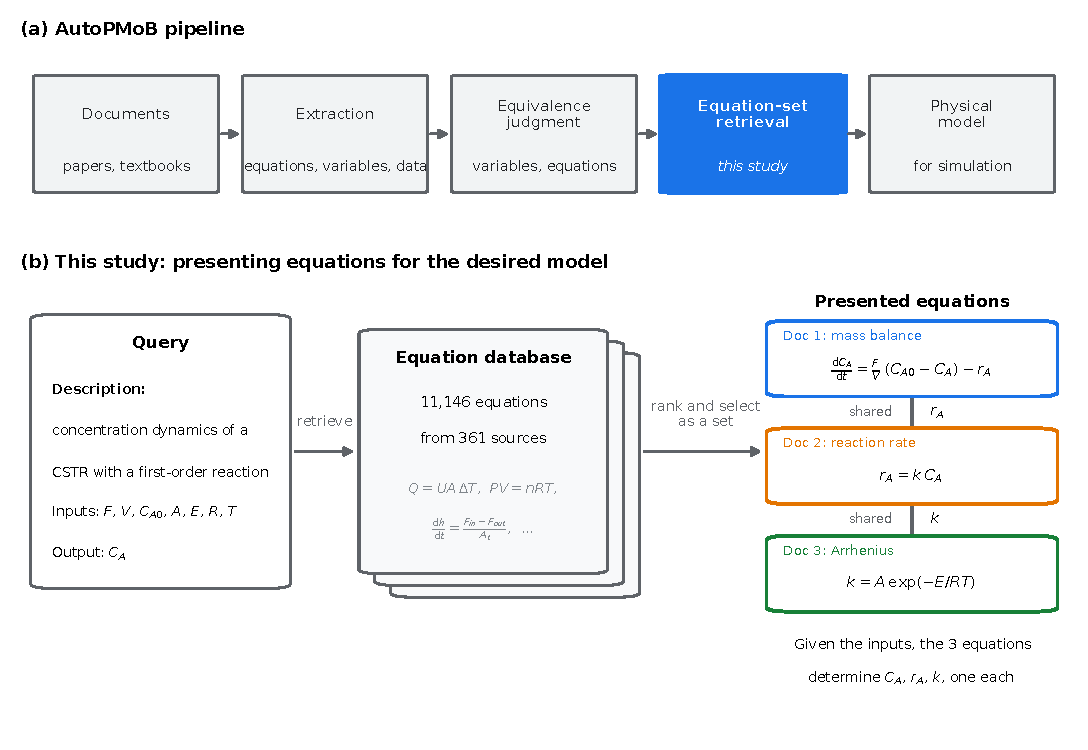
\includegraphics[width=0.98\linewidth]{figures/fig_autopmob_overview.pdf}
\caption{The automated physical model builder (AutoPMoB) and the position of this study. (a)
AutoPMoB collects documents about a target process, extracts equations, variables, and data,
judges their equivalence across documents, and reorganizes them into the desired model; this study
addresses the highlighted stage. (b) The task of this study: a query gives a description of the
desired model with its input and output variables, and the method presents, from a database of
equations extracted from many documents, the equations likely to serve in the model. The three
presented equations come from different documents and are linked by the variables they share
($r_A$ and $k$); once the inputs are given, they determine the three unknowns $C_A$, $r_A$, and
$k$, one equation each.}
\label{fig:overview}
\end{figure}

This study addresses the step that precedes the combination: given a description of the desired
model together with its input and output variables, present the equations likely to serve in the
model, drawn from a large equation database built from many documents
(Fig.~\ref{fig:overview}(b)). The aim is to present equations that are likely to be usable, not a
finished model; the engineer assembles and checks the model from them. The step is a retrieval
problem whose candidates depend on one another. A physical model is a set of equations from which
the output variables can be computed once the input variables are given, so an equation that
contains a variable other than the inputs and outputs is useful only together with an equation that
determines that variable. The concentration dynamics of a continuous stirred-tank reactor, for
example, need three equations: the mass-balance ordinary differential equation for the
concentration, the reaction-rate equation $r_A = k C_A$, and the Arrhenius equation
$k = A\exp(-E/RT)$ for the rate constant. The differential equation alone leaves the rate $r_A$
undetermined, the rate equation alone leaves the rate constant $k$ undetermined, and only the three
together determine the concentration from the inputs. A method that scores each equation by its
similarity to the description cannot see these dependencies. Retrieval must therefore evaluate
candidate equations as a set, not one by one.

We propose \ours{} (two-stage retrieval with attribute-conditioned evaluation). The first stage
ranks the whole database by a mixture of text similarity and variable overlap and keeps the top
candidates. The second stage evaluates each candidate again, conditioned on three attributes of an
equation: its variable set, its domain label, and its text. A multilayer perceptron reads ten
features of these attributes: seven compare a candidate with the query, and three, the set-aware
features, compare it with a reference set of equations. The set-aware features ask whether the
candidate supplies query variables that the reference set still lacks, whether it shares variables
with the set, and whether it carries the same domain label. A learned greedy variant builds the
ranking one equation at a time and compares each candidate with the equations already selected.

To evaluate the method, we built a database of \NEq{} equations: \NEqPdf{} that a large language
model (LLM) extracted from \NPdf{} PDF files of papers, textbooks, and reports, and \NEqRef{} that
it generated to cover textbook fundamentals. We also built \NCases{} cases, each a query with a
ground-truth equation set that meets the input--output and degree-of-freedom requirements of
\citet{CombineEq}. We split the cases by source into training,
validation, and test cases, repeat every experiment over 10 stratified splits, and choose the
hyperparameters on the validation cases.

\ours{} outperforms classical retrieval. Recall@20, the fraction of the ground-truth
equations among the 20 equations presented, rises from \RecABase{} to \RecAProp{} on all cases and
from \RecBBase{} to \RecBProp{} on the \NSynth{} cases that a program synthesized, in all 10 splits,
and the gain grows with the numbers of ground-truth equations and input variables. Ablation and
permutation importance locate the cause in the variables that the query and the equations share,
not in their topic.
We also compare the method with LLMs that receive the whole database and select equations without
training. The larger model, Claude Opus~5.5, reaches a Recall@20 of \RecAOpus{} and beats classical
retrieval, but \ours{} beats it in every split, by the widest margins on models that
combine several sources or many equations.

The contributions of this study are fourfold:
\begin{enumerate}
  \item a formulation of equation selection for physical model building as the retrieval of an
    equation set, with a benchmark of \NEq{} equations and \NCases{} cases split by source;
  \item \ours, a two-stage retrieval method with attribute-conditioned evaluation that improves
    Recall@20 and mean average precision over classical retrieval in every split;
  \item an empirical account of the method: which features cause the improvement, where
    sequential selection helps, why topical similarity adds little, and where the remaining errors
    arise;
  \item a comparison with LLMs that read the whole database, which identifies the strengths and
    weaknesses of the two approaches in accuracy, cost, and repeatability.
\end{enumerate}
